\chapter{Implementazione}
L'architettura software del progetto sviluppato è composta da tre moduli principali:
\begin{enumerate}
\item il compilatore offline, che comprende un compilatore per il linguaggio di specifica e il preprocessing dei pattern space;
\item la macchina diagnostica greedy, che rappresenta il motore diagnostico greedy;
\item la macchina diagnostica lazy, che attua la tecnica di ricostruzione lazy.
\end{enumerate}

La specifica dell'istanza di un sistema attivo complesso di cui si vuole determinare le diagnosi è espressa tramite un linguaggio creato ad hoc, la cui grammatica è fornita nell'appendice \ref{bnf}. Un esempio di specifica, relativo al problema diagnostico \ref{ex:prob_diagn}, è riportato nell'appendice \ref{spec_ex}.
Durante la lettura del file di specifica, sono generate le classi opportune e sono effettuati i controlli del caso. Se questa procedura di compilazione non contiene errori (lessicali, sintattici o semantici), viene effettuato il preprocessing offline del problema, durante il quale si creano gli automi relativi ai pattern space. Tutte le informazioni ottenute vengono salvate su appositi file, in modo che non sia necessario dover effettuare nuovamente la procedura in fase di lavoro online, ovvero quando viene avviata la macchina diagnostica, sia essa in modalità greedy o lazy. 
La procedura diagnostica legge i file generati da una precedente compilazione della specifica  e genera le soluzioni candidate. 
Il linguaggio di programmazione adottato è il C++, che è stato scelto in quanto buon compromesso tra le esigenze di efficienza richieste dal problema e il livello di astrazione tipico della programmazione ad oggetti.

\section{Rappresentazione degli automi}
Per la rappresentazione degli automi è stata ricercata una libreria esterna che fornisse da un lato delle strutture dati e dei metodi efficienti, dall'altro che fosse quanto più generica e personalizzabile, dal momento che gli automi necessari alle tecniche risolutive possiedono vari tipi di informazione negli stati e nelle transizioni. La libreria ASTL(\emph{Automata Standard Template Library})\cite{web:astl} soddisfa entrambe le esigenze. Le due classi principali di questa libreria utilizzate nell'implementazione sono:
\begin{itemize}
\item \verb|DFA_map<SIGMA,TAG>| rappresenta automi deterministici ed è implementata memorizzando le transizioni di uno stato in uno standard \verb|map|, associando i relativi simboli dell'alfabeto agli stati raggiunti. Dato che la struttura \verb|map| costituisce un albero binario, le operazioni di accesso, inserimento e cancellazione sono effettuate in un tempo logaritmico $\mathcal{O}(\log n)$ rispetto al numero di elementi contenuti.  Si tratta di un buon compromesso tra tempi richiesti dalle operazioni e memoria occupata.
\item \verb|NFA_mmap<SIGMA,TAG>|, rappresenta automi non deterministici. Le transizioni sono memorizzate per mezzo di \verb|multimap|, le cui principali operazioni hanno complessità logaritmica.
\end{itemize}
Il template \verb|SIGMA| permette di specificare l'alfabeto cui i simboli di transizione appartengono, mentre il template \verb|TAG| consente di associare ad uno stato delle informazioni satelliti generiche. 
Per la visualizzazione degli automi, in fase di debug nonché per le illustrazioni di questa trattazione, sono stati utilizzati metodi che generano file scritti nel linguaggio \verb|dot|, interpretati dal programma \emph{Graphviz}\cite{web:graphviz} che ne genera la rappresentazione.

\section{Classi condivise}
I tre moduli che compongono l'architettura software ideata hanno delle classi tra loro condivise, in modo da operare sulle stesse strutture dati. Si tratta di quegli oggetti che sono creati in fase di compilazione del file di specifica e che successivamente sono utilizzati al fine di avere le informazioni necessarie nella fase diagnostica.
Nel seguito vengono descritte tali classi.
\begin{itemize}

\item \verb|ComponentModel|\\ 
Rappresenta il modello di un componente. Ha come attributi la stringa del nome che lo identifica e vettori di stringhe contenenti i nomi di eventi, terminali di input, terminali di output e stati. Possiede un vettore di oggetti \verb|Transition| che contengono le informazioni relative ad ogni transizione del modello. L'attributo \verb|automaton| indica l'automa risultante dal modello comportamentale descritto dalle transizioni. Si noti che l'automa non è provvisto di stato iniziale, in quanto questa informazione è definitiva solo nella specifica del problema diagnostico.

\item \verb|NetComponent|\\
Rappresenta un componente generico nel modello di un nodo. Ha come attributi il nome, che lo identifica nel particolare modello di nodo nel quale è contenuto, e un riferimento ad un oggetto \verb|ComponentModel| che ne rappresenta il modello topologico e comportamentale.

\item \verb|Component|\\
Rappresenta un componente concreto del problema diagnostico. \'E una classe derivata da \verb|NetComponent| e possiede gli attributi aggiuntivi relativi all'automa ottenuto dal modello di componente associato, con l'informazione addizionale dello stato iniziale, e gli oggetti \verb|Terminal| riferiti ai terminali di input e output della sua topologia.

\item \verb|NetworkModel|\\
Rappresenta il modello di un nodo. Possiede gli attributi seguenti:
\begin{itemize}
\item \verb|name|: nome che identifica il modello del nodo;
\item \verb|components|: vettore di oggetti \verb|NetComponents| contenuti nel modello;
\item \verb|inputs| e \verb|outputs|: specificano i nomi dei terminali di input e dei terminali di output del modello del nodo;
\item \verb|links|: contiene l'elenco dei link che connettono tra loro i componenti e i terminali di input del nodo ai terminali di input dei componenti che gestiscono i pattern event in ingresso;
\item \verb|patterns|: vettore di oggetti di tipo \verb|Pattern|, ognuno dei quali rappresenta una dichiarazione di un pattern event che è generato in corrispondenza di un terminale di output del nodo;
\item \verb|initials|: nomi degli stati iniziali per ogni componente del nodo;
\item \verb|viewer|: \verb|map| tra nomi di transizioni di componenti e corrispondenti label osservabili;
\item \verb|ruler|: \verb|map| tra nomi di transizioni di componenti e corrispondenti label di guasto;
\item \verb|pattern_space|: vettore di automi che costituiscono i pattern space del nodo;
\item \verb|languages|: vettore di linguaggi, ognuno dei quali costituito da un insieme di stringhe recanti i nomi delle transizioni appartenenti al linguaggio di una o più dichiarazioni di pattern.
\end{itemize}
Si noti che le informazioni relative agli stati iniziali, al viewer e al ruler possono non essere presenti oppure venire sovrascritte nelle successive dichiarazioni di istanza del nodo del sistema o del problema diagnostico.
\item \verb|Pattern|\\
Rappresenta una dichiarazione di pattern e contiene gli attributi relativi al nome del pattern event, all'espressione regolare, al nome del terminale di destinazione del pattern event, un attributo booleano che indica se il linguaggio associato al pattern è massimo, ovvero costituito dall'insieme di tutte le transizioni di tutti i componenti del nodo, e un vettore di elementi del linguaggio.
\item \verb|Terminal|\\
rappresenta un terminale di un componente o di un nodo. \'E caratterizzato da una stringa del nome, una relativa al valore contenuto (evento), e un vettore di riferimenti a terminali ad esso connessi.
\item \verb|Transition|\\ 
Rappresenta la transizione di un modello di componente. Ha come attributi la stringa relativa al suo nome identificativo, una coppia di stringhe indicanti il nome dell'evento in ingresso e il terminale di input, un vettore di coppie di stringhe indicanti il nome dell'evento di uscita e il terminale di output, e la coppia del nome di stati sorgente-destinazione coinvolti nella transizione. 
Possiede attributi e metodi (l'operatore di confronto e di uguaglianza) in modo da permetterne l'utilizzo come alfabeto di un automa della libreria ASTL, come mostrato in figura \ref{class_trans}.
\item \verb|NetTransition|\\
Rappresenta la transizione di un componente del modello di un nodo. Ha come attributi il riferimento alla transizione del modello di componente del particolare componente del nodo, e un riferimento a quest'ultimo. Il nome è ottenuto, per mezzo del costruttore dell'oggetto, concatenando il nome della transizione associata e, tra parentesi, il nome del componente del nodo associato.
\item \verb|SysTransition|\\
Rappresenta la transizione di un componente concreto di un nodo del problema diagnostico. \'E una classe derivata da \verb|NetTransition| e presenta i seguenti attributi aggiuntivi:
\begin{itemize}
\item \verb|node|: il riferimento nodo del sistema relativo alla transizione;
\item \verb|input_event|: una coppia formata dal nome di un evento e dall'indice della tupla di terminali di input dei componenti del sistema (utile per la diagnosi greedy);
\item \verb|output_events|: un vettore di coppie formate dal nome di un evento e dall'indice della tupla di terminali di input dei componenti del sistema (utile per la diagnosi greedy);
\item \verb|lazy_input_event|: una coppia formata dal nome di un evento e dall'indice della tupla di terminali di input dei componenti del nodo coinvolto (utile per la diagnosi lazy);
\item \verb|lazy_output_events|: un vettore di coppie formate dal nome di un evento e dall'indice della tupla di terminali di input dei componenti del nodo coinvolto (utile per la diagnosi lazy).
\end{itemize}
\item \verb|System|\\
Rappresenta la specifica del sistema. Possiede i seguenti attributi:
\begin{itemize}
\item \verb|name|: nome del sistema;
\item \verb|node_list|: vettore dei nodi del sistema;
\item \verb|emergence|: lista delle dichiarazioni di link tra nodi del sistema;
\item \verb|dependency_graph|: grafo che rappresenta la topologia del sistema;
\item \verb|acyclic|: attributo booleano di valore \verb|true| se la topologia del sistema è aciclica e permette quindi la diagnosi lazy.
\end{itemize}
\item \verb|SystemNode|\\
Rappresenta un nodo del sistema ed è caratterizzato da un nome identificativo e un riferimento all'oggetto di tipo \verb|NetworkModel| che ne costituisce il modello; possiede inoltre gli attributi relativi agli stati iniziali dei suoi componenti, al viewer e al ruler locali, i quali possono essere ereditati dal modello o sovrascritti nella specifica del problema diagnostico.
\item \verb|Problem|\\
Rappresenta il problema diagnostico e possiede un nome, una lista di nodi del problema e un vettore di indici  che indica l'ordinamento topologico dei nodi, al fine di poter effettuare la diagnosi lazy.
\item \verb|ProblemNode|\\
Rappresenta un nodo del problema diagnostico. Possiede i seguenti attributi:
\begin{itemize}
\item \verb|name|: nome del nodo, ottenuto dal nodo del sistema associato;
\item \verb|ref_node|: riferimento al nodo del sistema;
\item \verb|concrete_components|: vettore di componenti concreti;
\item \verb|input_terminals|: vettore di terminali di ingresso fisici del nodo;
\item \verb|output_terminals|: vettore di terminali di uscita fisici del nodo;
\item \verb|observation|: sequenza di label relative all'osservazione locale;
\item \verb|index_space|: automa lineare ottenuto dall'osservazione, utile per eventuali sviluppi futuri nei quali l'osservazione è incerta;
\item \verb|depends|: lista di indici dei nodi dai quali il nodo corrente dipende topologicamente;
\item \verb|patt_map|: mappa un pattern event nel terminale di uscita fisico del nodo;
\item \verb|patt_indexes_map|: mappa un pattern event nell'indice della tupla dei terminali di input dei componenti dell'intero problema (utile per la diagnosi greedy);
\item \verb|lazy_patt_indexes_map|: mappa un pattern event nell'indice della tupla dei terminali di input dei componenti del nodo (utile per la diagnosi lazy);
\end{itemize}
La classe contiene inoltre le informazioni definitive riguardanti gli stati iniziali dei componenti, il viewer e il ruler locali, che possono essere ereditati dalla specifica del nodo del sistema.
\item \verb|Utils|, contiene metodi statici di utilità.
\end{itemize}


\begin{figure}[htbp]
\begin{verbatim}
class Transition : public CHAR_TRAITS<Transition>
{
    ...
    //required definitions to use a Transition 
    //as automata alphabet for ASTL lib
    typedef Transition char_type;
    typedef long        int_type;
    static const size_t size;
    static bool eq(const char_type &x, const char_type &y) 
    { return x == y; }
    static bool lt(const char_type &x, const char_type &y) 
    { return x < y; }
    bool operator<(const Transition t) const {return name<t.name;}
    bool operator==(const Transition t) const {return name == t.name;}
};
\end{verbatim}
\caption{Classe Transition}
\label{class_trans}
\end{figure}

In figura \ref{fig:comp} è riportato il diagramma UML delle classi relative ai componenti del sistema, ovvero le classi \verb|ComponentModel|, \verb|NetComponent| e \verb|Component|.\\
In figura \ref{fig:trans} è riportato il diagramma UML delle classi relative alle transizioni, ovvero \verb|Transition|, \verb|NetTransition| e \verb|SysTransition|.\\
In figura \ref{fig:nodes} è riportato il diagramma UML delle classi che rappresentano, nei diversi livelli di definizione, i nodi del sistema, cioè le classi \verb|NetworkModel|, \verb|SystemNode| e \verb|ProblemNode|.

\begin{figure}[htbp]
\centering
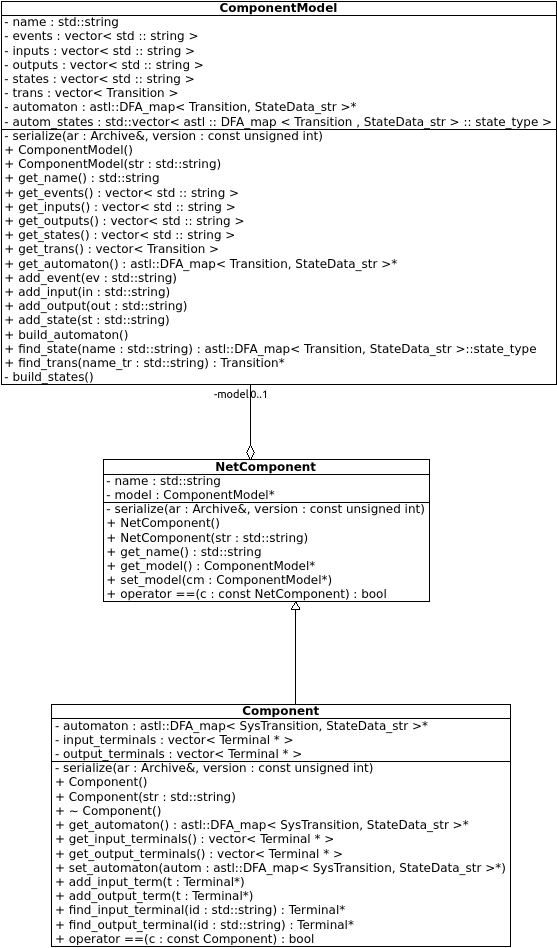
\includegraphics[scale=0.6]{./Img/implementazione/comp.png}
\caption{Classi dei componenti}
\label{fig:comp}
\end{figure}

\begin{figure}[htbp]
\centering
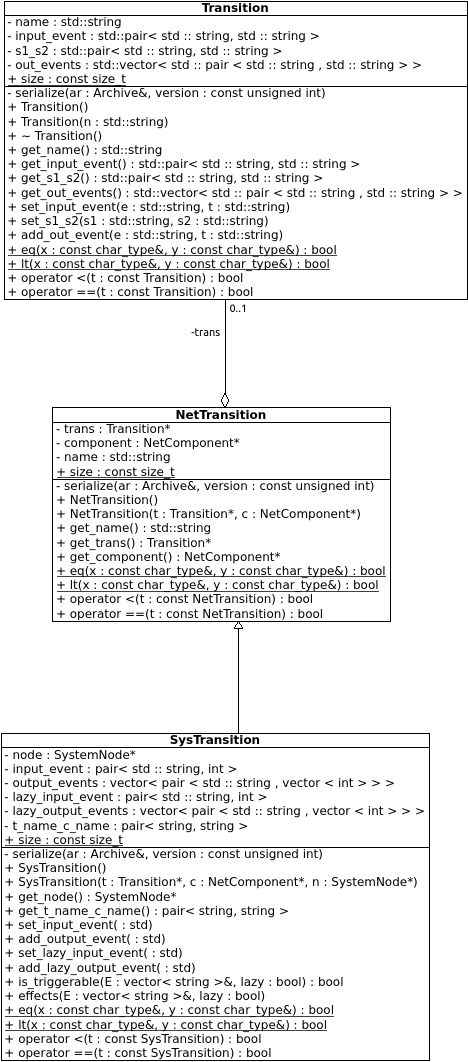
\includegraphics[scale=0.6]{./Img/implementazione/trans.png}
\caption{Classi delle transizioni}
\label{fig:trans}
\end{figure}

\begin{figure}[htbp]
\centering
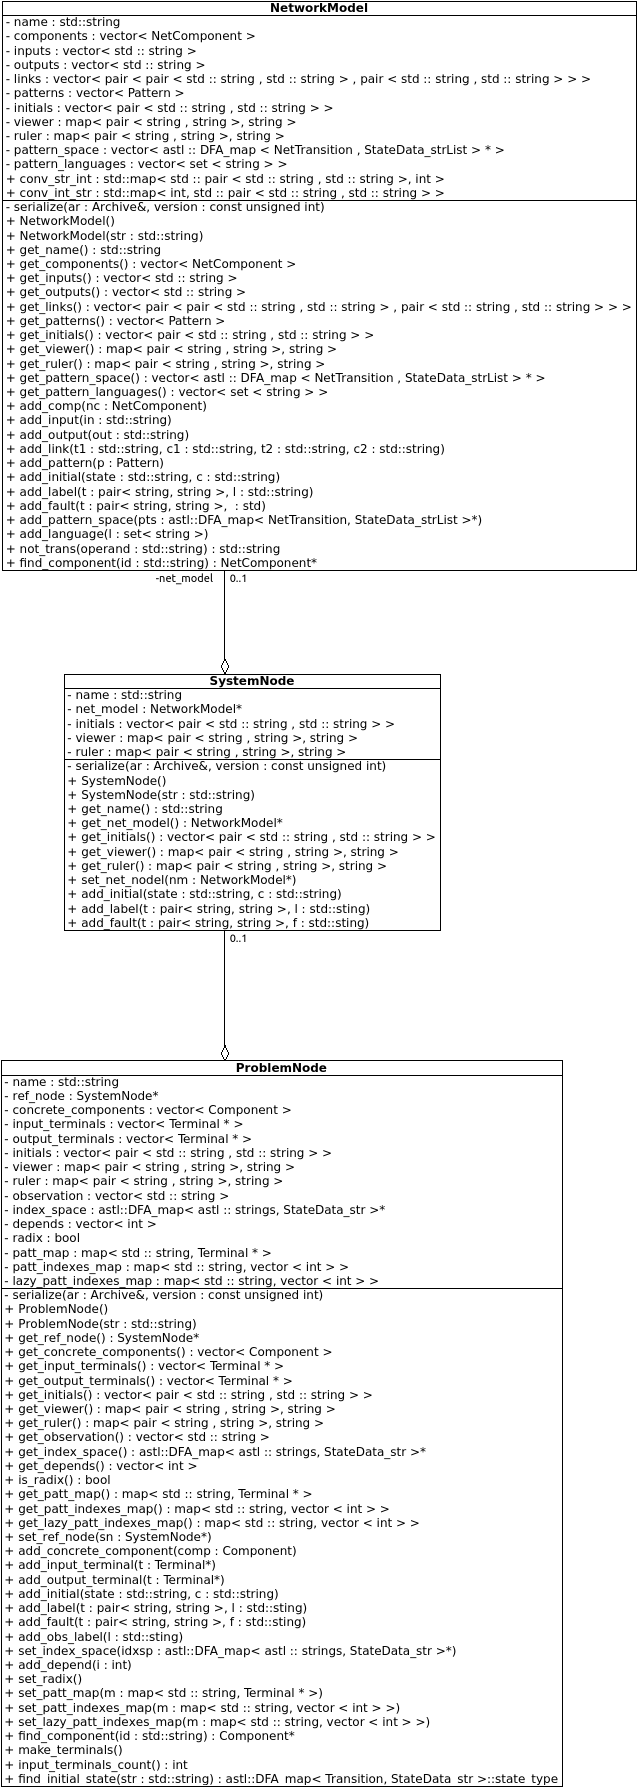
\includegraphics[scale=0.45]{./Img/implementazione/nodes.png}
\caption{Classi dei nodi}
\label{fig:nodes}
\end{figure}

\newpage
\section{Compilatore offline}
Il linguaggio di specifica dei sistemi attivi complessi è fornito, tramite notazione BNF, in appendice \ref{bnf}. 
Il file di specifica è articolato in quattro parti principali:
\begin{itemize}
\item modelli dei componenti, a cui i componenti concreti del sistema si riferiscono;
\item modelli dei nodi, a cui i nodi concreti del sistema si riferiscono;
\item sistema, che istanzia i nodi e definisce i link responsabili dell'invio di pattern event tra di essi;
\item problema, che fornisce informazioni necessarie per il problema diagnostico, come le osservazioni locali dei nodi.
\end{itemize}
I viewer locali, i ruler locali e gli stati iniziali dei componenti dei singoli nodi possono essere definiti, con eventuale riscrittura, a tre diversi livelli:
\begin{itemize}
\item nella definizione del modello del nodo;
\item nella dichiarazione di un nodo del sistema;
\item nella specifica di un nodo del problema.
\end{itemize}
Questo permette una certa facilità di scrittura, non essendo costretti a dichiarare informazioni di questo tipo, quando esse sono ridondanti.
Il file di specifica viene compilato seguendo le tradizionali fasi ideate per i compilatori dei linguaggi di programmazione:
\begin{enumerate}
\item analisi lessicale, che legge il flusso di caratteri che costituiscono il codice di specifica e raggruppa i caratteri in sequenze significative dette lessemi, quali le parole chiave del linguaggio e gli identificatori;
\item analisi sintattica, che riceve i lessemi dall'analizzatore lessicale per creare una rappresentazione ad albero del codice di specifica, detto albero sintattico;
\item analisi semantica, la quale utilizza le informazioni raccolte nell'albero sintattico in modo da verificare la consistenza del codice di specifica.
\end{enumerate}
Si noti che in questo progetto è possibile articolare una specifica in più file, esplicitando delle dichiarazioni del tipo \verb|#include| per i file che si vogliono incorporare. 
Questo permette il riutilizzo di specifiche già dichiarate precedentemente, aumentando inoltre la leggibilità dei file di specifica.


\subsection{Analizzatore lessicale}
L'analizzatore lessicale (o scanner) è implementato mediante lo strumento \emph{Flex}, il quale permette di dichiarare espressioni regolari che descrivono i pattern per i token, ovvero coppie nome-attributo, ad esempio \verb|<id,breaker>|. La struttura di un programma Flex  è composta da tre parti principali:
\begin{enumerate}
\item dichiarazioni, che includono variabili, costanti e definizioni regolari;
\item regole di traduzione, che specificano per ogni pattern dichiarato per mezzo di una espressione regolare le azioni da compiere, attraverso frammenti di codice;
\item funzioni ausiliarie, che possono essere richiamate nelle azioni dei pattern.
\end{enumerate}
Sebbene Flex abbia un'opzione per creare direttamente uno scanner C++, il codice generato spesso non funziona e contiene errori\cite{book:bison} .
La procedura adottata per risolvere questo problema è quella di compilare il programma Flex scritto in linguaggio C per mezzo di un compilatore C++.
La sezione dichiarativa del linguaggio è riportata in figura \ref{code:lex_decl}. In essa si definiscono spazi, delimitatori, commenti di linea (in stile C) e l'espressione regolare che definisce gli identificatori \verb|id|, formata da una lettera a cui seguono altre lettere, numeri oppure il carattere \verb|_|.

\begin{figure}[htbp]
\begin{verbatim}
// The location of the current token.
yy::location loc;

%}
%option noyywrap nounput
%x incl

delimiter	[ \t]
spacing		{delimiter}+
letter		[A-Za-z]
digit		[0-9]
unscore         _
id		{letter}({letter}|{digit}|{unscore})*
eol		\n
comment		\/\/.*

%{
  // Code run each time a pattern is matched.
  # define YY_USER_ACTION  loc.columns (yyleng);
%}
\end{verbatim}
\caption{Dichiarazioni.}
\label{code:lex_decl}
\end{figure}

Le regole di traduzione utilizzate sono principalmente volte a generare i token relativi a parole chiave del linguaggio e agli identificatori.
In corrispondenza di direttive \verb|#include|, il passaggio di lettura al file incluso è operato, come mostrato in figura \ref{code:lex_rules}, creando una pila di buffer. 

\begin{figure}[htbp]
\begin{verbatim}
#include          BEGIN(incl);
<incl>[ \t]*      /* eat the whitespace */
<incl>[^ \t\n]+   
{   /* got the include file name */
    chdir(INPUT_FILE_DIR);
    FILE *file = fopen( yytext, "r" );

    if (file == NULL)
    {
       cout << "Input file error: included file does not exist" << endl;
       exit(1);
    }
    yyin = file;

    yypush_buffer_state(yy_create_buffer( yyin, YY_BUF_SIZE ));
    BEGIN(INITIAL);
}
\end{verbatim}
\caption{Gestione delle direttive di inclusione.}
\label{code:lex_rules}
\end{figure}

Gli spazi e i commenti non invocano alcuna azione, mentre la fine del file attuale toglie dalla pila il buffer corrente, riportando il controllo alla scansione del file precedente da cui la direttiva di inclusione è stata chiamata (figura \ref{code:lex_buff}). Se il buffer corrente è l'unico elemento della pila, il processo di scanning termina ed è generato il token relativo alla fine del file.

\begin{figure}[htbp]
\begin{verbatim}
{spacing}	;
{comment}   ;

{eol}		{loc.lines (yyleng);loc.step();}

<<EOF>>    
{
  yypop_buffer_state();
  if ( !YY_CURRENT_BUFFER )
    return yy::spec_parser::make_END_OF_FILE(loc);;
  
}
\end{verbatim}
\caption{Azioni compiute alla fine del file.}
\label{code:lex_buff}
\end{figure}

Quando viene trovata una parola chiave (come ad esempio \verb|component| e \verb|model|), viene creato il corrispondente token che verrà utilizzato nell'analisi sintattica.
Per quanto riguarda gli identificatori (\verb|id|), il loro token è composto oltre che dalla posizione, dalla stringa che ne rappresenta il nome, memorizzato durante lo scanning nella variabile \verb|yytext| (figura \ref{code:lex_id}).
La lettura di un carattere non appartenente a nessuna delle configurazioni definite genera un errore lessicale.

\begin{figure}[htbp]
\begin{verbatim}
component   return yy::spec_parser::make_COMPONENT(loc);
model       return yy::spec_parser::make_MODEL(loc);
is          return yy::spec_parser::make_IS(loc);


{id}        return yy::spec_parser::make_ID(yytext,loc);
.		    {cout << "Lexical error"; exit(1);}
\end{verbatim}
\caption{Regole di traduzione per parole chiave e identificatori.}
\label{code:lex_id}
\end{figure}

\subsection{Analizzatore sintattico}
L'analizzatore sintattico (parser) è implementato tramite lo strumento \emph{Bison}. La generazione della grammatica è supportata dalla classe \verb|spec_driver|, la quale avvia il parsing e ne gestisce gli eventuali errori generati.
Il file della grammatica inizia richiedendo lo skeleton parser deterministico per poter utilizzare direttamente il linguaggio C++, creando il file header della grammatica e specificando il nome della classe del parser.

\begin{verbatim}
%skeleton "lalr1.cc"
%defines
%define parser_class_name {spec_parser}
\end{verbatim}

Per poter utilizzare oggetti C++ come valori semantici della grammatica, deve essere richiesta l'interfaccia \verb|variant|.

\begin{verbatim}
%define api.value.type variant
%define api.token.constructor
%define parse.assert
\end{verbatim}
 
Successivamente sono specificate le dichiarazioni necessarie ai valori semantici. Poiché il parser utilizza la classe driver e viceversa, questa mutua dipendenza è risolta fornendo una \emph{forward declaration}. 

\begin{verbatim}
%code requires
{
...
class spec_driver;
}
\end{verbatim}

L'oggetto driver viene passato al parser e allo scanner tramite referenza.

\begin{verbatim}
%param { spec_driver& driver}
\end{verbatim}

Quindi viene richiesto di tenere traccia della locazione (riga e colonna del file di specifica), passando il nome del file dell'oggetto \verb|driver|.

\begin{verbatim}
%locations
%initial-action
{
  // Initialize the initial location.
  @$.begin.filename = @$.end.filename = &driver.file;
};
\end{verbatim}

La definizione dei token avviene come di seguito.

\begin{verbatim}
%token
COMPONENT
MODEL
IS
...
END_OF_FILE  0  "end of file"
COMMA ","
...
\end{verbatim}

Per ogni terminale e non terminale della grammatica, deve essere specificato un tipo dell'oggetto.

\begin{verbatim}
%token <string> ID "id"
%type <ComponentModel>  comp_model_decl
%type <vector<string> > event_decl
..
\end{verbatim}

Successivamente viene implementata la grammatica del linguaggio, assegnando i valori semantici definiti.

\subsection{Analizzatore semantico}
L'analisi semantica, a differenza di quella lessicale e sintattica, non prevede l'utilizzo di strumenti standard per la sua attuazione, ma è compito del programmatore definirne le regole, in base al significato del linguaggio specificato Nell'ambito di questo progetto, i controlli semantici sono affidati alla classe \verb|spec_driver| (figura \ref{fig:driver}), la quale verifica la consistenza semantica durante il parsing del file, interrompendone l'esecuzione in caso di errori. 

\begin{figure}[htbp]
\centering
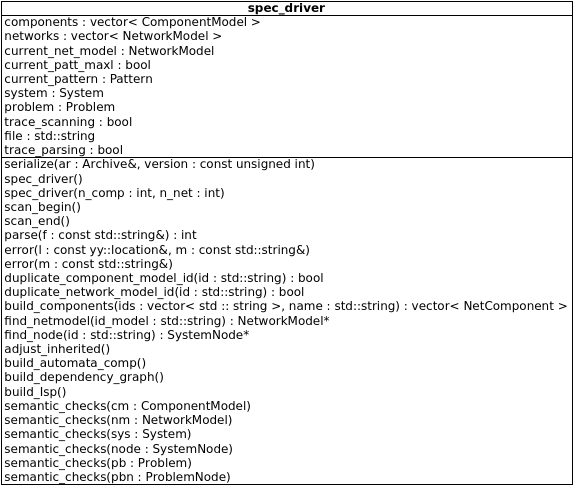
\includegraphics[scale=0.7]{./Img/implementazione/driver.png}
\caption{Classe specdriver}
\label{fig:driver}
\end{figure}

La classe possiede, tra gli altri, i metodi \verb|semantic_checks|, implementati in \emph{overloading} per i seguenti tipi di parametro d'ingresso:
\begin{enumerate}
\item \verb|ComponentModel|: verifica che non vi siano identificatori multipli per le liste di eventi, terminali di input, terminali di output e stati; nelle dichiarazioni delle transizioni, verifica che il nome degli eventi, dei terminali e degli stati siano stati precedentemente definiti. 
\item \verb|NetworkModel|: verifica l'unicità del nome dei componenti, dei terminali e dei nomi dei pattern;
verifica che i terminali e i componenti dei link siano definiti. Verifica che non vi siano più link entranti nello stesso terminale di input. Verifica l'esistenza delle transizioni utilizzate nei pattern, nel viewer e nel ruler (se presenti), oltre all'esistenza degli eventuali stati iniziali dei componenti dichiarati.
\item \verb|System|: verifica che nelle dichiarazioni di \emph{emergence} i nomi dei nodi e dei relativi terminali siano stati definiti.
\item \verb|SystemNode|: effettua i controlli sulle eventuali dichiarazioni di stati iniziali, viewer e ruler locali.
\item \verb|Problem|: verifica che siano ivi dichiarati tutti i nodi definiti nel sistema.
\item \verb|ProblemNode|: verifica i controlli sulle eventuali dichiarazioni di stati iniziali, viewer e ruler locali. Se esse non sono presenti, vengono ereditate dal nodo di sistema corrispondente. Viene inoltre verificata l'esistenza delle label dell'osservazione locale nel viewer corrente.
\end{enumerate}
L'analisi semantica viene ultimata, attraverso il metodo \verb|build_dependency_graph|, costruendo il grafo che rappresenta la topologia del sistema, verificando che sia connesso. La connessione è verificata nel metodo \verb|Utils::disconnected_graph|, il quale compie un'intera traversata in ampiezza del grafo; se il numero di nodi visitati è inferiore al numero di nodi dichiarati, alcuni di essi non sono connessi. 
Viene inoltre verificata l'aciclicità del grafo, eliminando uno dopo l'altro i nodi foglia dal grafo, fino a quando esso non risulta essere vuoto. Se ad un certo punto della procedura non vi sono nodi foglia e il grafo non è vuoto, significa che sono presenti ciclicità e non sarà possibile avviare la diagnosi lazy.
Nel caso il grafo sia aciclico, viene calcolato l'ordinamento topologico, attraverso un algoritmo simile al precedente. 

\subsection{Generazione dei pattern space}
La principale azione compiuta in fase offline, ovvero in un momento antecedente la diagnosi, è la generazione dei pattern space dei modelli di nodi definiti, come descritto nel paragrafo \ref{pts_construction}. 
Il primo passo di questo algoritmo consiste nella costruzione di un automa equivalente all'espressione regolare definita nella dichiarazione di pattern. Un metodo noto consiste nella costruzione di Thompson descritta nel paragrafo \ref{thompson}. 
Per questo scopo, è stata utilizzata la libreria \emph{Grail+}\cite{web:grail}, una libreria C++ che permette di definire espressioni regolari e convertirle in automi con un linguaggio equivalente.
La conversione avviene utilizzando la sintassi presentata in figura \ref{code:patodfa}.

\begin{figure}[htbp]
\begin{verbatim}
fm<int> patodfa(std::string regex)
{
    re<int> r;
    istringstream str(regex);
    str >> r;
    fm<int> dfa;
    r.retofm(dfa);
    dfa.subset();

    return dfa;
}
\end{verbatim}
\caption{Passaggio da espressione regolare ad automa}
\label{code:patodfa}
\end{figure}

Data una stringa in ingresso, la funzione implementata inserisce tale stringa in un oggetto della classe \verb|re|(\emph{regular expression}), parametrizzato per mezzo di un template che indica l'alfabeto di appartenenza dei simboli dell'espressione. 
Dato che gli alfabeti possibili per questa libreria erano esclusivamente di tipo \verb|char| o \verb|int|, è stato scelto quest'ultimo (poiché 256 simboli possibili potevano non essere sufficienti in applicazioni di dimensioni ragguardevoli), mantenendo una corrispondenza biunivoca tra ogni intero e una transizione, coinvolta nella dichiarazione del pattern, relativa ad un componente del nodo. La conversione da espressione regolare ad automa a stati finiti avviene applicando all'oggetto che rappresenta l'espressione regolare il metodo \verb|retofm|, che crea l'automa nell'oggetto della classe \verb|fm|(\emph{finite machine}) passato come parametro. A seguito della conversione, l'automa è determinizzato applicando il metodo \verb|subset|, il quale esegue la subset construction descritta nel paragrafo\ref{subset}.
Successive manipolazioni dei diversi automi ottenuti dai pattern dichiarati permettono di unirli, aggiungere le $\epsilon$-transizioni opportune e determinizzare il risultato. L'automa finale viene poi convertito in un automa equivalente, utilizzando le strutture dati della libreria ASTL. Infatti, la libreria Grail+, sebbene utile poiché implementa la costruzione di Thompson, non sembrava indicata ad un utilizzo negli algoritmi di diagnosi, in quanto non permette estensioni per quanto riguarda i dati satellite associati a transizioni e stati dell'automa.
La minimizzazione finale del pattern space è implementata nel metodo \verb|Utils::minimize_by_partition|, che esegue una minimizzazione tenendo conto dei tag associati (pattern event) ai nodi finali dell'automa.

\subsection{Salvataggio dei dati compilati}
Una volta che il file di specifica è stato processato, le classi opportune sono state create e i controlli semantici sono andati a buon fine, la procedura di elaborazione offline termina creando dei file binari contenenti tutte le informazioni utili alla successiva fase diagnostica, ovvero tutti gli oggetti istanziati per il problema specificato. La scrittura di questi dati, chiamata serializzazione, è una procedura piuttosto complessa se implementata manualmente in C++, in quanto deve gestire puntatori ed evitare ridondanza. Per questo è stata adottata la libreria \emph{Serialization}, fornita dalla collezione \emph{Boost}\cite{web:boost}. Essa permette di salvare un oggetto con semplici modifiche della classe a cui esso appartiene.
Ad esempio, la definizione della classe \verb|ComponentModel| è stata modificata aggiungendo le istruzioni riportate in figura \ref{code:serialize}. Per ogni attributo della classe, viene specificata la lettura e la scrittura in un oggetto di tipo \verb|Archive|, appartenente alla libreria. \'E necessario esplicitare l'operazione per ogni attributo della classe, in modo da poter salvare lo stato dell'oggetto corrente; eventuali attributi non salvati avranno un valore impredicibile. Quando l'oggetto corrisponde ad un archivio di output, l'operatore \verb|&| indica la scrittura, mentre nel caso di un archivio di input esso indica l'operazione di lettura. Le modifiche attuate permettono quindi sia la scrittura su file che la lettura operata durante la successiva fase diagnostica.

\begin{figure}[htbp]
\begin{verbatim}
#include <boost/archive/text_oarchive.hpp>
#include <boost/archive/text_iarchive.hpp>

class ComponentModel{
    friend class boost::serialization::access;
    template<class Archive>
    void serialize(Archive & ar, const unsigned int version)
    {
        ar & autom_states;
        ar & name;
        ar & automaton;
        ar & events;
        ar & inputs;
        ar & outputs;
        ar & states;
        ar & trans;
    }
\end{verbatim}
\caption{Modifiche apportate alla classe ComponentModel per la serializzazione.}
\label{code:serialize}
\end{figure}

Il programma sviluppato salva le informazioni precompilate in quattro file distinti:
\begin{itemize}
\item un file contenente tutti i modelli dei componenti (\verb|component_models.dat|);
\item un file che comprende tutti i modelli dei nodi (\verb|network_models.dat|);
\item un file che racchiude la specifica del sistema (\verb|system.dat|);
\item un file contenente le informazioni del problema diagnostico con le osservazioni temporali (\verb|problem.dat|).
\end{itemize}
Per eseguire la scrittura di un oggetto è sufficiente dare istruzioni simili a quelle riportate in figura \ref{code:serialize_main}, nella quale è salvato su file il \verb|vector| dei modelli dei componenti utilizzati nel sistema.

\begin{figure}[htbp]
\begin{verbatim}
{
    std::ofstream ofs("../../CompiledData/component_models.dat");
    boost::archive::text_oarchive oa(ofs);
    // write class instance to archive
    oa << driver.components;
    // archive and stream closed when destructors are called
}
\end{verbatim}
\caption{Serializzazione.}
\label{code:serialize_main}
\end{figure}

Si noti che la libreria \emph{Serialization} permette di salvare, senza il bisogno di istruzioni aggiuntive, oggetti appartenenti alla Standard Template Library, quali ad esempio \verb|vector|, \verb|map|, \verb|list| e \verb|set|. Per quanto riguarda il salvataggio di puntatori, al fine di evitare ridondanza, la libreria salva l'oggetto puntato un'unica volta, mantenendone i riferimenti.


\section{Macchina diagnostica}

\subsection{Lettura dei dati precompilati}
La fase diagnostica necessita degli oggetti generati dal precedente passo di compilazione dei file di specifica. La lettura delle informazioni salvate avviene in modo simile a quanto fatto per la scrittura, come si può vedere in figura \ref{code:read_files}.


\begin{figure}[htbp]
\begin{verbatim}
vector<ComponentModel> components;
{
    // create and open an archive for input
    std::ifstream ifs("../../CompiledData/component_models.dat");
    boost::archive::text_iarchive ia(ifs);
    // read class state from archive
    ia >> components;;
    // archive and stream closed when destructors are called
}
\end{verbatim}
\caption{Lettura dai file binari e memorizzazione degli oggetti salvati.}
\label{code:read_files}
\end{figure}

\subsection{Modalità greedy}
La modalità greedy implementa l'algoritmo di ricostruzione del behavior dell'intero sistema. Dopo aver acquisito gli oggetti memorizzati nei file precompilati, viene generato lo stato iniziale con i seguenti campi:
\begin{itemize}
\item una tupla di interi indicanti gli stati iniziali di tutti i componenti del problema;
\item una tupla di stringhe recanti il valore, inizialmente vuoto, del contenuto dei terminali di input di tutti i componenti del sistema;
\item una tupla di interi indicanti gli stati iniziali di tutti i pattern space di ogni nodo;
\item una tupla di interi indicanti gli stati iniziali degli index space di ogni nodo (osservazione locale, inizialmente nulla).
\end{itemize} 
La classe che rappresenta uno stato del behavior è riportata in figura \ref{fig:bhv_state}.

\begin{figure}[htbp]
\centering
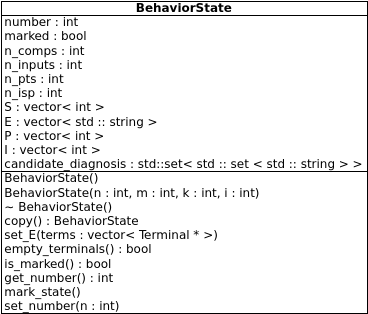
\includegraphics[scale=0.7]{./Img/implementazione/bhv_state.png}
\caption{Classe BehaviorState}
\label{fig:bhv_state}
\end{figure}

L'algoritmo tiene traccia delle configurazioni di ogni stato attraverso una tabella hash: in questo modo la verifica dell'esistenza di uno stato generato da una transizione avviene in tempo costante. La tabella mappa la stringa relativa al contenuto dello stato nel valore intero associato allo stato del behavior, come mostrato di in figura \ref{code:hash_tab} per lo stato iniziale.

\begin{figure}[htbp]
\begin{verbatim}
DFA_map<SysTransition,BehaviorState> behavior;
unordered_map<string,unsigned int> hash_values;
stringstream ss;
ss << tag_s0;
unsigned int s0 = behavior.new_state();
behavior.tag(s0) = tag_s0;
behavior.initial(s0);
hash_values[ss.str()] = s0;
\end{verbatim}
\caption{Creazione tabella hash}
\label{code:hash_tab}
\end{figure}

La creazione del behavior avviene come descritto nella sezione \ref{section_greedy}.
La verifica dell'esistenza di uno stato raggiunto da una transizione avviene come descritto in figura \ref{code:ricerca_hash}, dove \verb|tag_s1| è un'istanza della classe \verb|BehaviorState|.

\begin{figure}[htbp]
\begin{verbatim}
stringstream s_str;
s_str << tag_s1;
string str = s_str.str();
unsigned int s1;
try{ s1 = hash_values.at(str);}
catch (const std::out_of_range&)
{
    s1 = behavior.new_state();
    behavior.tag(s1) = tag_s1;
    hash_values[str] = s1;
...
\end{verbatim}
\caption{Ricerca nella tabella hash}
\label{code:ricerca_hash}
\end{figure}

Per ogni stato creato viene contestualmente verificato se si tratta di uno stato finale, ovvero caratterizzato da terminali di input vuoti e che ha consumato tutte le osservazioni locali dei vari nodi.
Una volta terminato il ciclo principale della generazione del behavior, ed ottenuto quindi il behavior spurio, esso viene potato di tutte le transizioni e gli stati che non sono in un cammino tra lo stato iniziale ed uno stato finale. L'operazione avviene invocando la funzione predisposta \verb|trim| presente nella libreria ASTL (figura \ref{code:trim}).

\begin{figure}[htbp]
\begin{verbatim}
DFA_map<SysTransition,BehaviorState> bhv;
unsigned int init = trim(bhv,dfirst_markc(behavior));
\end{verbatim}
\caption{Rimozione della parte spuria del behavior}
\label{code:trim}
\end{figure}

Se dopo questa operazione il behavior risulta vuoto, significa che le osservazioni date non sono consistenti con il modello specificato e l'esecuzione viene terminata con errore. Questo può avvenire in fase di sperimentazione, a causa dell'assenza di un reale sistema fisico che dia un'osservazione vera del comportamento.
Altrimenti, l'algoritmo procede decorando l'automa ottenuto e distillandone le diagnosi.
L'algoritmo di decorazione consiste nella semplice implementazione dello pseudocodice \ref{alg:decoration}. La distillazione consiste nell'unione delle diagnosi contenute negli stati finali del behavior.

\subsection{Modalità lazy}
La diagnosi lazy avviene in maniera simile alla ricostruzione greedy, con alcune variazioni. 
Viene letto l'ordinamento topologico del sistema e viene applicata in successione la ricostruzione del comportamento del singolo nodo. Ogni nodo che non è l'ultimo dell'ordinamento topologico, ovvero che non costituisce un nodo radice, necessita della generazione della sua interfaccia. Durante la generazione dei behavior, si tiene conto anche delle dipendenze dalle interfacce dei nodi inferiori collegati al nodo corrente.


\subsubsection{Determinizzazione dell'interfaccia}
La classe \verb|Determinization| fornisce dei metodi statici che permettono di ottenere l'interfaccia associata al behavior locale di un nodo. 
\'E composta dai metodi seguenti:
\begin{itemize}
\item \verb|NFAtoDFA| guida il processo di determinizzazione, ricevendo il behavior del nodo;
\item \verb|eps_closure| calcola la $\epsilon$-chiusura di uno stato o di un insieme di stati del behavior, nel quale le transizioni che non producono pattern event sono sostituite da $\epsilon$-transizioni;
\item \verb|extract_subNFA| estrae dall'automa del behavior la parte contenente gli stati appartenenti alla $\epsilon$-chiusura, in modo che tale sottoautoma possa essere memorizzato nello stato dell'interfaccia;
\item \verb|move| calcola gli stati raggiungibili attraverso transizioni, applicate a stati interni allo stato dell'interfaccia, che generano pattern event.
\end{itemize}
La decorazione del sottoautoma contenuto negli stati dell'interfaccia avviene richiamando un metodo della classe \verb|Decoration| che implementa la classica decorazione come nell'algoritmo \ref{alg:decoration}.
La classe che rappresenta lo stato dell'interfaccia è visualizzata in figura \ref{fig:int_state}.
Le transizioni dell'interfaccia (figura \ref{fig:int_trans}) possiedono invece i seguenti attributi:
\begin{itemize}
\item \verb|trans|: transizione di un componente del nodo;
\item \verb|delta|: diagnosi associata alla transizione;
\item \verb|pattern_events|: elenco dei patter event associati alla transizione dell'interfaccia.
\end{itemize}

\begin{figure}[htbp]
\centering
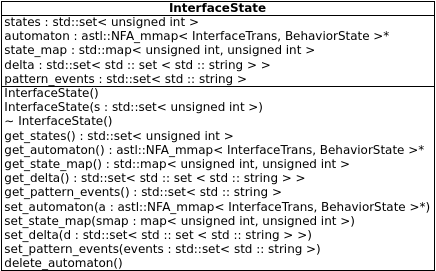
\includegraphics[scale=0.7]{./Img/implementazione/int_state.png}
\caption{Classe InterfaceState}
\label{fig:int_state}
\end{figure}

\begin{figure}[htbp]
\centering
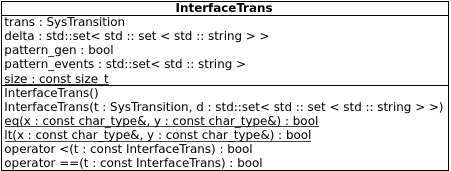
\includegraphics[scale=0.7]{./Img/implementazione/int_trans.png}
\caption{Classe InterfaceTrans}
\label{fig:int_trans}
\end{figure}

\subsubsection{Decorazione del behavior del nodo radice}
La decorazione del behavior del nodo radice avviene attraverso il metodo \verb|decorate_lazy_bhv| della classe \verb|Decoration|. La procedura consiste in alcune variazioni dell'algoritmo di decorazione della diagnosi greedy:
\begin{itemize}
\item una transizione del behavior, se relativa ad una interfaccia, contiene una diagnosi che deve essere propagata agli stati successivi;
\item in corrispondenza di uno stato finale del behavior, la decorazione deve tenere conto delle diagnosi relative agli stati finali delle interfacce da cui il nodo corrente dipende.
\end{itemize}